
% v2-acmsmall-sample.tex, dated March 6 2012
% This is a sample file for ACM small trim journals
%
% Compilation using 'acmsmall.cls' - version 1.3 (March 2012), Aptara Inc.
% (c) 2010 Association for Computing Machinery (ACM)
%
% Questions/Suggestions/Feedback should be addressed to => "acmtexsupport@aptaracorp.com".
% Users can also go through the FAQs available on the journal's submission webpage.
%
% Steps to compile: latex, bibtex, latex latex
%
% For tracking purposes => this is v1.3 - March 2012
\documentclass[prodmode,acmtecs]{acmsmall} % Aptara syntax
\usepackage[spanish,polish]{babel}
\usepackage[T1]{fontenc}
\usepackage{fancyvrb}
\usepackage{graphicx,hyperref}
\newcommand\cutout[1]{}


\usepackage[table]{xcolor}
\usepackage[utf8]{inputenc}
\usepackage[parfill]{parskip}
\usepackage{tabulary}
\PassOptionsToPackage{hyphens}{url}
\usepackage{hyperref}    
\usepackage[capitalize]{cleveref}


% Metadata Information
% !!! TODO: SET THESE VALUES !!!
\acmVolume{0}
\acmNumber{0}
\acmArticle{CFP}
\acmYear{0}
\acmMonth{0}

\newcounter{colstart}
\setcounter{page}{4}

\RecustomVerbatimCommand{\VerbatimInput}{VerbatimInput}%
{
%fontsize=\footnotesize,
fontfamily=\rmdefault
}


\newcommand{\UnderscoreCommands}{%\do\verbatiminput%
\do\citeNP \do\citeA \do\citeANP \do\citeN \do\shortcite%
\do\shortciteNP \do\shortciteA \do\shortciteANP \do\shortciteN%
\do\citeyear \do\citeyearNP%
}

\usepackage[strings]{underscore}



% Document starts
\begin{document}


\setcounter{colstart}{\thepage}

\acmArticle{CFP}
\title{\huge\sc SIGLOG Monthly 218}
\author{DAVID PURSER\affil{Max Planck Institute for Software Systems, Saarbr\"ucken}
\vspace*{-2.6cm}\begin{flushright}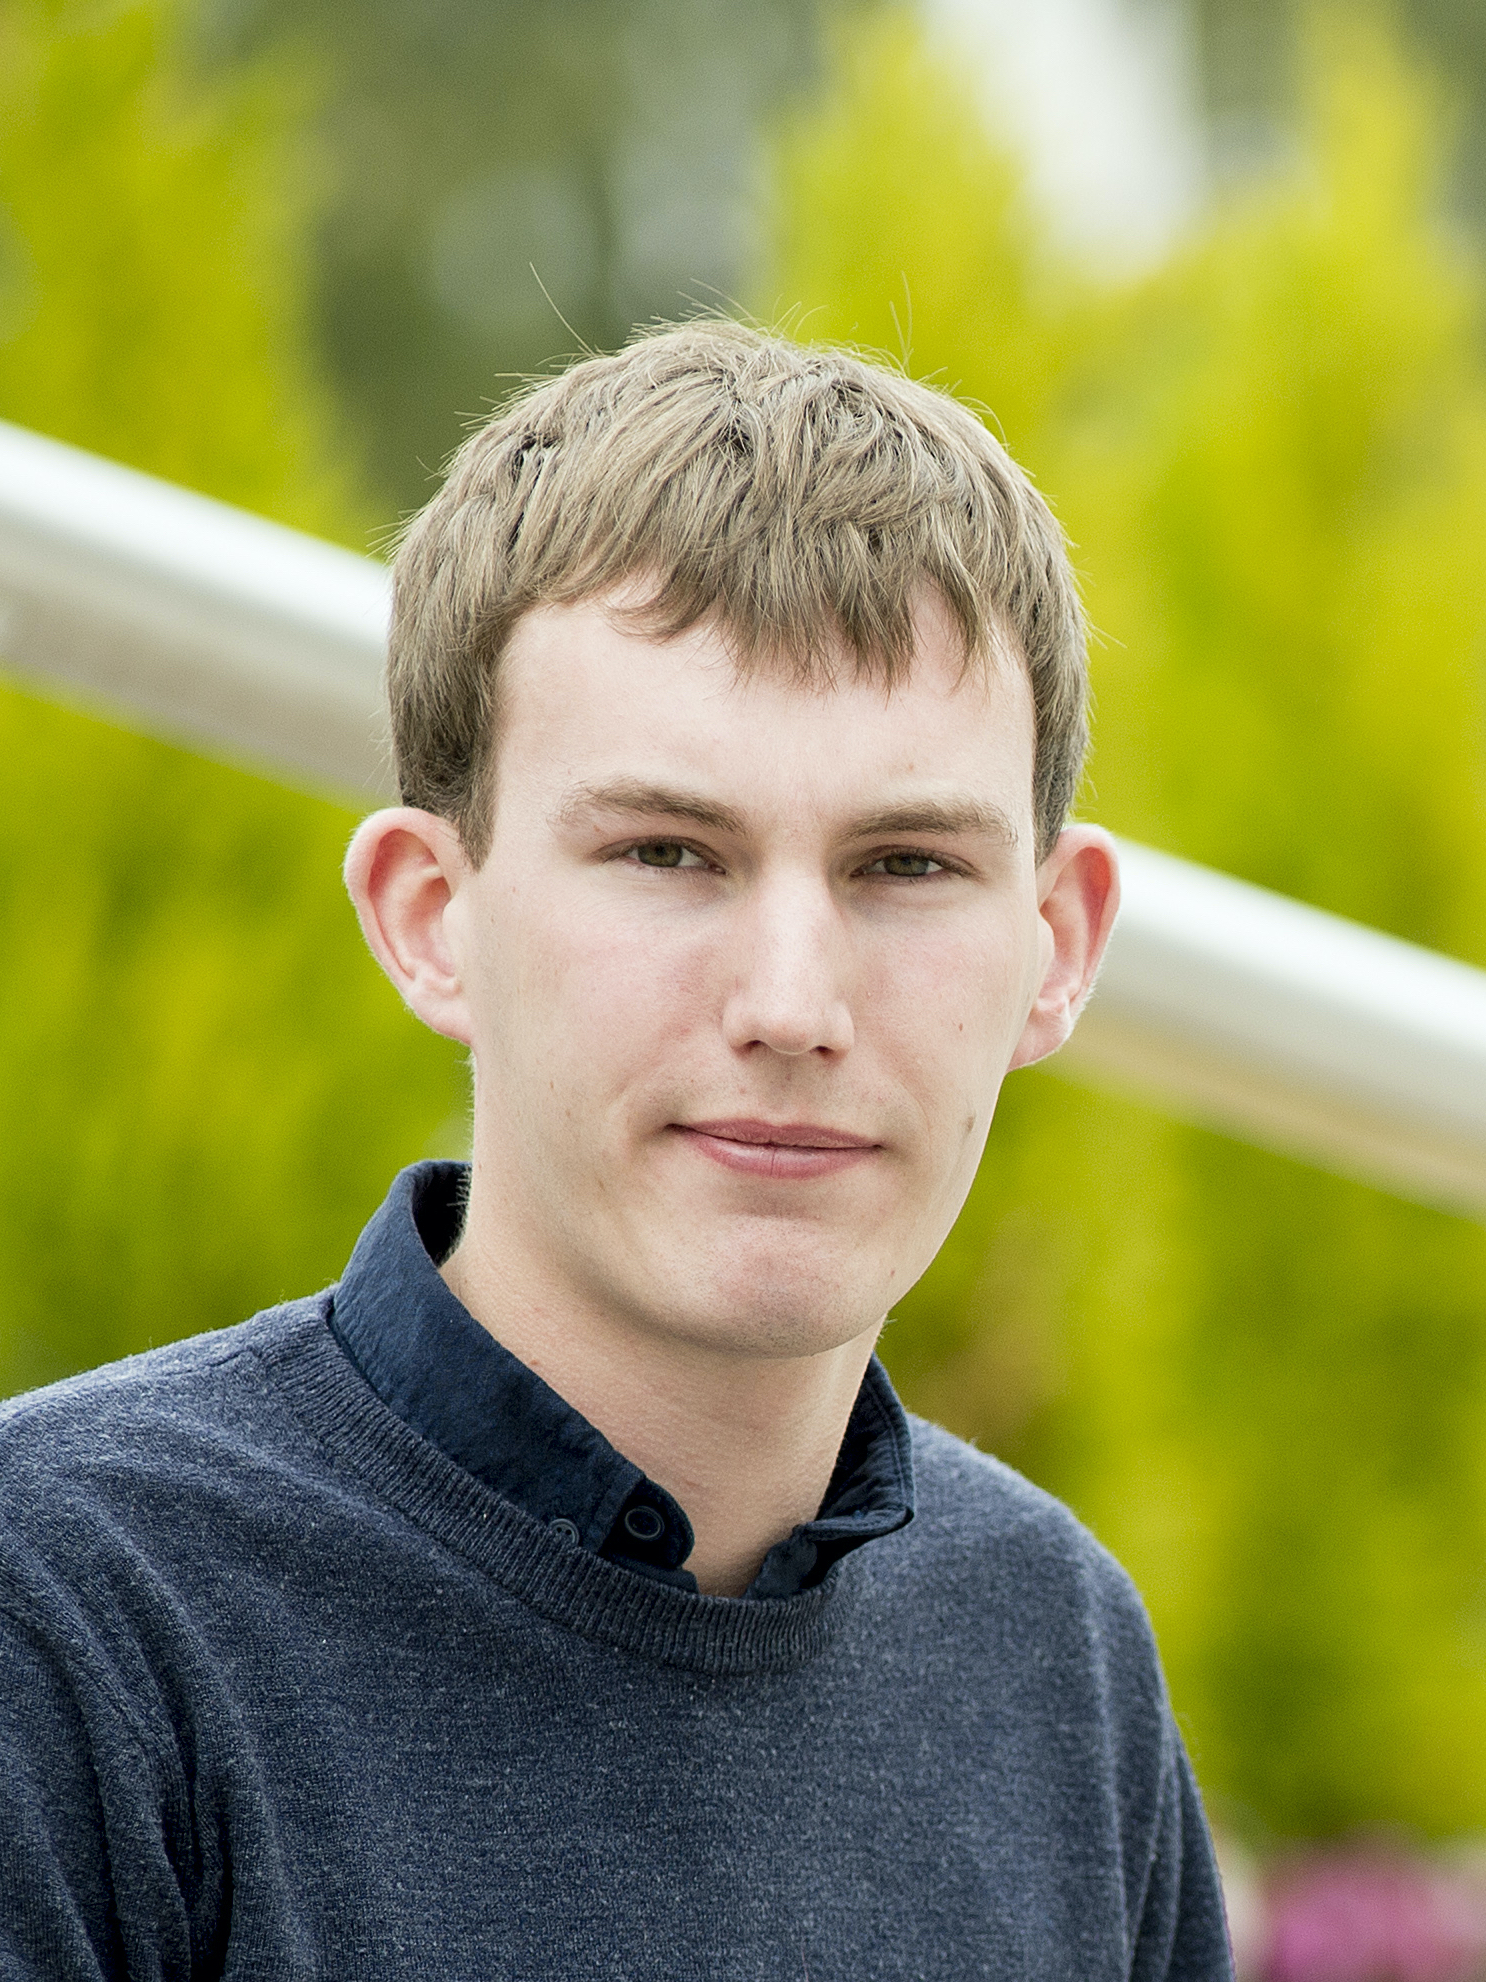
\includegraphics[width=30mm]{dp}\end{flushright}
}

\maketitlee

\href{https://lics.siglog.org/newsletters/}{Past Issues}
 - 
\href{https://lics.siglog.org/newsletters/inst.html}{How to submit an announcement}
\section{Table of Content}\begin{itemize}\item DEADLINES (\cref{deadlines}) 
 
\item CALLS 
 
\begin{itemize}\item HyLo 2022 (CALL FOR PAPERS) (\cref{HyLo2022})
\item ICALP 2022 (CALL FOR WORKSHOPS) (\cref{ICALP2022})
\item NFM 2022 (CALL FOR PAPERS) (\cref{NFM2022})
\item FSCD 2022 (CALL FOR PAPERS) (\cref{FSCD2022})
\item AiML 2022 (CALL FOR PAPERS) (\cref{AiML2022})
\end{itemize} 
\end{itemize}\section{Deadlines}\label{deadlines}\rowcolors{1}{white}{gray!25}\begin{tabulary}{\linewidth}{LL}HyLo 2022:  & Oct 09, 2021 (Abstract  deadline) \\
HSCC 2022:  & Oct 29, 2021 (Submission deadline) \\
ICALP 2022:  & Nov 19, 2021 (Workshop proposal deadline) \\
NFM 2022:  & Dec 03, 2021 (Abstract), Dec 10, 2021 (Paper) \\
FSCD 2022:  & Feb 08, 2022 (Abstract), Feb 11, 2022 (Paper) \\
AiML 2022:  & Mar 07, 2022 (Abstracts for full papers), Mar 14, 2022 (Full papers), May 23, 2022 (Short presentations) \\
\end{tabulary}
\section{HyLo 2022: Workshop on Hybrid Logic and Applications }\label{HyLo2022}  April 6-11, 2022, Crete, Greece\\ 
  \href{https://sites.google.com/view/unilog-2022/workshops/hybrid-logic}{https://sites.google.com/view/unilog-2022/workshops/hybrid-logic}\\ 
CALL FOR PAPERS 

\begin{itemize}\item  IMPORTANT DATES 
 
\rowcolors{1}{white}{gray!25}\begin{tabulary}{\linewidth}{LL}Abstract submission deadline:  & Oct 09, 2021 \\
Notification:  & Oct 21, 2021 \\
Worskhop:  & Apr 6-11, 2022 \\
\end{tabulary}
 
\item  Target audience: Logicians (computational, philosophical, mathematical) 
 
\item  Hybrid logic is a branch of modal logic in which it is possible to directly refer to worlds/times/states or whatever the elements of the (Kripke) model are meant to represent. Hybrid logic is now a mature field with significant impact on a range of other fields, including  
 
\begin{itemize}\item  applied modal logics,
\item  temporal logic,
\item  labelled deduction,
\item  philosophy of time, and
\item  social reasoning.
\end{itemize} 
\item  The scope of the workshop is not only standard hybrid-logical machinery like nominals, satisfaction operators, and the downarrow binder, but generally extensions of modal logic that increase its expressive power. 
 
\item  The duration of the workshop is a half day or one day and it will take place at some point during the UNILOG congress, April 6-11, 2022. 
 
\end{itemize}\section{ICALP 2022: International Colloquium on Automata, Languages and Programming}\label{ICALP2022}  July 4 - July 8, 2022\\ 
  Paris, France\\ 
  \href{https://icalp2022.irif.fr/}{https://icalp2022.irif.fr/}\\ 
CALL FOR WORKSHOPS 

\begin{itemize}\item  The International Colloquium on Automata, Languages and Programming (ICALP) is the main conference and annual meeting of the EATCS (European Association for Theoretical Computer Science). This year, after two virtual ICALP events, we are happy to be able to host this event in hybrid mode--and hope that many of us will be able to meet again in beautiful Paris!  This is a call for workshops to be affiliated with ICALP 2022. We invite researchers to organise workshops on central topics on Automata, Languages and Programming, to help further mark off ICALP 2022.  
 
\item  Important Dates (Aoe) 
 
\rowcolors{1}{white}{gray!25}\begin{tabulary}{\linewidth}{LL}Workshop proposal deadline:  & Nov 19, 2021 \\
Workshop notification:  & Dec 10, 2021 \\
Workshops:  & Jul 04, 2022 \\
\end{tabulary}
 
\item  Workshop Proposal Guidelines: 
 
  We strongly suggest that prospective workshop organizers contact the workshop selection committee before submitting a proposal. 
 
  Proposals should be submitted  by sending an email to the workshop selection committee. You should expect notification on the acceptance of your proposal by 10 December 2021. 
 
\item  A workshop proposal submission should consist of the following  
 
  A short scientific justification of the proposed topic, its significance, and the particular benefits of the workshop to the community. 
 
  An organisational part including: 
 
\begin{itemize}\item  workshop’s name and URL (if already available);
\item  contact information for the workshop organizers (including their webpages);
\item  expected number of participants (if available, please include the data of previous years);
\item  proposed format and agenda (e.g. paper presentations, tutorials, see below for more details);
\item  potential invited speakers;
\item  plans for dissemination, if any (e.g. a journal special issue);
\item  planned format of the event (see below for mode details);
\item  virtual/hybrid backup plans (including platform preference).
\end{itemize} 
  As for the format, a standard option is a full one-day workshop consisting of invited talks by leading experts and of shorter contributed talks, either directly invited by the organizers or selected among presentation submissions. Deviations from this standard are also welcome, including open problem sessions, discussion panels, or working sessions. If you plan to have invited speakers, please specify their expected number and, if possible, tentative names. If you plan a call for contributed talks (or papers) followed by a selection procedure, the submission date should be scheduled after ICALP 2022 notification (11 April 2022), while the notification should take place before the early registration deadline. In your submission please include details on the schedule, planned procedure of selecting contributed talks (or papers). If you plan to have published proceedings of your workshop, please provide the name of the publisher. 
 
  Note that ICALP 2022 is not able to provide financial support for the organization of workshops.  The conference can however provide a room, internet connection and help with some local organisation.  For workshops that are online or in hybrid mode, it is expected that the organizers provide the supporting technical infrastructure.  
 
\item  Workshop Selection Committee:  
 
\begin{itemize}\item  Track A:  Valia Mitsou vmitsou@irif.fr
\item  Track B:  Mahsa Shirmohammadi mahsa@irif.fr
\end{itemize} 
\end{itemize}\section{NFM 2022: The 14th NASA Formal Methods Symposium}\label{NFM2022}  \href{https://shemesh.larc.nasa.gov/nfm2022/}{https://shemesh.larc.nasa.gov/nfm2022/}\\ 
  May 24-27, 2022\\ 
  Pasadena, California, USA\\ 
CALL FOR PAPERS 

\begin{itemize}\item  The symposium is planned to be held in person at California Institute of Technology, but potentially transitioning to fully virtual if the COVID situation persists. Virtual presentations will be possible even if the conference is held in-person. 
 
  The symposium has NO registration fee for presenting and attending. 
 
\item  IMPORTANT DATES 
 
\rowcolors{1}{white}{gray!25}\begin{tabulary}{\linewidth}{LL}Abstract submission:  & Dec 03, 2021 \\
Paper submission:  & Dec 10, 2021 \\
Paper Notifications:  & Feb 04, 2022 \\
Camera-ready Papers:  & Mar 04, 2022 \\
Symposium:  & May 24-27, 2022 \\
\end{tabulary}
 
\item  THEME OF SYMPOSIUM 
 
  The widespread use and increasing complexity of mission-critical and safety-critical systems at NASA and in the aerospace industry requires advanced techniques that address these systems' specification, design, verification, validation, and certification requirements. The NASA Formal Methods Symposium (NFM) is a forum to foster collaboration between theoreticians and practitioners from NASA, academia, and industry. NFM's goals are to identify challenges and to provide solutions for achieving assurance for such critical systems. The focus of the symposium will be on formal/rigorous techniques for software assurance, including their theory, current capabilities and limitations, as well as their potential application to aerospace during all stages of the software life-cycle. 
 
  The NASA Formal Methods Symposium is an annual event organized by the NASA Formal Methods (NFM) Research Group, composed of researchers spanning six NASA centers. The organization of NFM 2022 is being led by the Jet Propulsion Laboratory (JPL), located in Pasadena, California. 
 
\item  TOPICS ON INTEREST 
 
  Topics of interest include, but are not limited to, the following aspects of formal methods: 
 
\begin{itemize}\item  Advances in formal methods: Interactive and automated theorem proving, SMT and SAT solving, Model checking , Static analysis, Runtime verification, Automated testing, Specification languages, textual and graphical , Refinement, Code synthesis , Design for verification and correct-by-design techniques, Requirements specification and analysis
\item  Integration of formal methods techniques: Integration of diverse formal methods techniques, Use of machine learning and probabilistic reasoning techniques in formal methods, Integration of formal methods into software engineering practices, Combination of formal methods with simulation and analysis techniques, Formal methods and fault tolerance, resilient computing, and self healing systems, Formal methods and graphical modeling languages such as SysML, UML, MATLAB/Simulink, Formal methods and autonomy, e.g., verification of systems and languages for planning and scheduling (PDDL, Plexil, etc.), self-sufficient systems, and fault-tolerant systems.
\item  Formal methods in practice: Experience reports of application of formal methods on real systems, such as autonomous systems, safety-critical systems, concurrent and distributed systems, cyber-physical, embedded, and hybrid systems, fault-detection, diagnostics, and prognostics systems, and human-machine interaction analysis, Use of formal methods in systems engineering (including hardware components), Use of formal methods in education, Reports on negative results in the development and the application for formal methods in practice., Usability of formal method tools, and their infusion into industrial contexts., Challenge problems for future reference by the formal methods community. The formulation of these papers can range from plain English description of a problem over formal specifications, to specific implementations in a programming language.
\end{itemize} 
\item  NASA OPEN SOURCE  
 
  Courageous authors, who want to delve in open source software being applied in real NASA missions, and find possible connections to and applications of Formal Methods, are invited to visit the open source repositories for the following two frameworks for programming flight software: F’ (\href{https://nasa.github.io/fprime/}{https://nasa.github.io/fprime/}) and cFS (\href{https://cfs.gsfc.nasa.gov/}{https://cfs.gsfc.nasa.gov/}). 
 
\item  SUBMISSIONS  
 
  There are two categories of submissions: 
 
\begin{itemize}\item  Regular papers describing fully developed work and complete results (maximum 15 pages, excluding references);
\item  Short papers on tools, experience reports, or work in progress with preliminary results (maximum 6 pages, excluding references).
\end{itemize} 
  Additional appendices can be submitted as supplementary material for reviewing purposes. They will not be included in the proceedings.   
 
  All papers must be in English and describe original work that has not been published. All submissions will be reviewed by at least three members of the Program Committee. We encourage authors to focus on readability of their submissions.  
 
  Papers must use LNCS style formatting and will appear in the Formal Methods subline of Springer's Lecture Notes in Computer Science (LNCS) PDF Submission: \href{https://easychair.org/conferences/?conf=nfm2022}{https://easychair.org/conferences/?conf=nfm2022}. 
 
  Authors of selected best papers will be invited to submit an extended version to a special issue in Springer's Innovations in Systems and Software Engineering: A NASA Journal (\href{https://www.springer.com/journal/11334}{https://www.springer.com/journal/11334}). 
 
\item  ARTIFACTS 
 
  Authors are encouraged, but not strictly required, to submit artifacts that support the conclusions of their work (if allowed by their institutions). Artifacts may contain software, mechanized proofs, benchmarks, examples, case studies and data sets. Artifacts will be evaluated by the Program Committee together with the paper.  
 
\end{itemize}\section{FSCD 2022: Seventh International Conference on Formal Structures for Computation and Deduction }\label{FSCD2022}  August 2-5, 2022, Haifa, Israel\\ 
  \href{https://fscd2022.github.io/}{https://fscd2022.github.io/}\\ 
  In-cooperation with ACM SIGLOG and SIGPLAN\\ 
CALL FOR PAPERS 

\begin{itemize}\item  IMPORTANT DATES (AoE) 
 
\rowcolors{1}{white}{gray!25}\begin{tabulary}{\linewidth}{LL}Abstract:  & Feb 08, 2022 \\
Paper submission:  & Feb 11, 2022 \\
Rebuttal:  & Mar 29-Apr 1, 2022 \\
Notification:  & Apr 15, 2022 \\
Final version:  & Apr 30, 2022 \\
\end{tabulary}
 
\item  FSCD (\href{http://fscd-conference.org/}{http://fscd-conference.org/}) covers all aspects of formal structures for computation and deduction from theoretical foundations to applications. Building on two communities, RTA (Rewriting Techniques and Applications) and TLCA (Typed Lambda Calculi and Applications), FSCD embraces their core topics and broadens their scope to closely related areas in logics, models of computation, semantics and verification in new challenging areas. 
 
\item  TOPICS  
 
  The suggested, but not exclusive, list of topics for submission is: 
 
\begin{itemize}\item  Calculi: Rewriting systems (string, term, higher-order, graph, conditional, modulo, infinitary, etc.); Lambda calculus; Logics (first-order, higher-order, equational, modal, linear, classical, constructive, etc.); Proof theory (natural deduction, sequent calculus, proof nets, etc.); Type theory and logical frameworks; Homotopy type theory; Quantum calculi.
\item  Methods in Computation and Deduction: Type systems (polymorphism, dependent, recursive, intersection, session, etc.); Induction, coinduction; Matching, unification, completion, orderings; Strategies (normalization, completeness, etc.); Tree automata; Model building and model checking; Proof search and theorem proving; Constraint solving and decision procedures.
\item  Semantics: Operational semantics and abstract machines; Game Semantics and applications; Domain theory and categorical models; Quantitative models (timing, probabilities, etc.); Quantum computation and emerging models in computation.
\item  Algorithmic Analysis and Transformations of Formal Systems: Type Inference and type checking; Abstract Interpretation; Complexity analysis and implicit computational complexity; Checking termination, confluence, derivational complexity and related properties; Symbolic computation.
\item  Tools and Applications: Programming and proof environments; Verification tools; Proof assistants and interactive theorem provers; Applications in industry; Applications of formal systems in other sciences.
\item  Semantics and Verification in new challenging areas: Certification; Security; Blockchain protocols; Data Bases; Deep learning and machine learning algorithms; Planning.
\end{itemize} 
\item  PUBLICATION 
 
  The proceedings will be published as an electronic volume in the Leibniz International Proceedings in Informatics (LIPIcs) of Schloss Dagstuhl. All LIPIcs proceedings are open access. 
 
\item  SPECIAL ISSUE 
 
  Authors of selected papers will be invited to submit an extended version to a special issue of Logical Methods in Computer Science. 
 
\item  SUBMISSION GUIDELINES  
 
  Submit in LIPIcs style at \href{https://easychair.org/conferences/?conf=fscd2022}{https://easychair.org/conferences/?conf=fscd2022} 
 
  Submissions can be made in two categories.  Regular research papers are limited to 15 pages, excluding references and appendices.  They must present original research which is unpublished and not submitted elsewhere.  System descriptions are limited to 15 pages, excluding references.  They must present new software tools, or significantly new versions of such tools, in which FSCD topics play an important role. An archive of the code with instructions on how to install and run the tool must be submitted.  In addition, a webpage where the system can be experimented with should be provided. 
 
  One author of an accepted paper is expected to present it at the (physical) conference, unless Covid restrictions prevent travel. 
 
\item  BEST PAPER AWARD BY JUNIOR RESEARCHERS 
 
  The program committee will select a paper in which at least one author is a junior researcher, i.e. either a student or whose PhD award date is less than three years from the first day of the meeting. Other authors should declare to the PC Chair that at least 50% of contribution is made by the junior researcher(s). 
 
\end{itemize}\section{AiML 2022: 14TH INTERNATIONAL CONFERENCE ON ADVANCES IN MODAL LOGIC}\label{AiML2022}  RENNES, AUGUST 22-25, 2022\\ 
  \href{http://www.aiml.net}{http://www.aiml.net}  \\ 
  Co-located with the Workshop on Logical Aspects of Multi-Agent Systems and Strategic Reasoning (LAMAS\&SR 2022).  \\ 
CALL FOR PAPERS 

\begin{itemize}\item  Advances in Modal Logic is an initiative aimed at presenting the state of the art in modal logic and its various applications. The initiative consists of a conference series together with volumes based on the conferences.  
 
\item  TOPICS  
 
  We invite submissions on all aspects of modal logic, including: 
 
\begin{itemize}\item  history of modal logic 
\item  philosophy of modal logic 
\item  applications of modal logic 
\item  computational aspects of modal logic (complexity and decidability of 
\item  modal and temporal logics, modal and temporal logic programming, 
\item  model checking, model generation, theorem proving for modal logics) 
\item  theoretical aspects of modal logic (topological/algebraic/categorical perspectives 
\item  on modal logic, coalgebraic modal logic, completeness and canonicity, 
\item  correspondence and duality theory, many-dimensional modal logics, 
\item  modal fixed point logics, model theory of modal logic, proof theory 
\item  of modal logic) 
\item  specific instances and variations of modal logic (description logics, 
\item  modal logics over non-boolean bases, dynamic logics and other process 
\item  logics, epistemic and deontic logics, modal logics for agent-based 
\item  systems, modal logic and game theory, modal logic and grammar 
\item  formalisms, provability and interpretability logics, spatial and 
\item  temporal logics, hybrid logic, intuitionistic logic, substructural 
\item  logics, computationally light fragments of all such logics) 
\end{itemize} 
  Papers on related subjects will also be considered.  
 
\item  PAPER SUBMISSIONS  
 
  There will be two types of submissions for AiML 2022:  
 
\begin{itemize}\item   Full papers for publication in the proceedings and presentation at the conference. 
\item  Short presentations intended for presentation at the conference but not for the published proceedings. 
\end{itemize} 
  Both types of papers should be submitted electronically using the EasyChair submission page which will be made available in due course.  
 
  At least one author of each accepted paper or short presentation must register for and attend the conference.  
 
\item  FULL PAPERS   
 
  Authors are invited to submit, for presentation at the conference and publication in the proceedings, full papers reporting on original research and not submitted elsewhere. Information on the submission procedure will be made available in due course.   
 
  The submissions should be at most 15 pages, with an optional technical appendix of up to 5 pages, together with a plain-text abstract of 100-200 words. The submissions must be typeset in LaTeX, using the style files and template that will be provided on the AiML 2022 website in due time.  
 
  Authors must submit an abstract in plain text via EasyChair by the abstract deadline prior to full submission of their paper.  
 
  The presentations of accepted full papers will be 30 minutes long.  
 
\item  SHORT PRESENTATIONS.  
 
  These should be at most 5 pages. They may describe preliminary results, work in progress etc., and will be subject to light reviewing. The accepted submissions will be made available at the conference, and the authors will have the opportunity to give short presentations (of up to 15 minutes) on them.  
 
\item  IMPORTANT DATES  
 
\rowcolors{1}{white}{gray!25}\begin{tabulary}{\linewidth}{LL}Abstracts for full papers submission:  & Mar 07, 2022 \\
Full papers submission:  & Mar 14, 2022 \\
Full papers acceptance notification:  & May 13, 2022 \\
Short presentations submission:  & May 23, 2022 \\
Short presentations acceptance notification:  & Jun 06, 2022 \\
Final version of full papers and short presentations due:  & Jun 13, 2022 \\
Conference:  & Aug 22-25, 2022 \\
\end{tabulary}
 
\end{itemize}


To the \href{http://siglog.org/}{SIGLOG} or \href{https://lics.siglog.org}{LICS} website\end{document}